\documentclass[a4paper]{article}

\usepackage{color}
\usepackage{xurl}
\usepackage[T2A]{fontenc} % enable Cyrillic fonts
\usepackage[utf8]{inputenc} % make weird characters work
\usepackage{csquotes}
\usepackage{graphicx}
\usepackage{subfigure}
\usepackage{float}
\usepackage[english,serbian]{babel}
\usepackage{listings}
\usepackage{amsthm}
\usepackage{amsmath}

\usepackage[unicode]{hyperref}
\hypersetup{colorlinks,citecolor=green,filecolor=green,linkcolor=blue,urlcolor=blue}


\newtheorem{theorem}{Theorem}[section]
\newtheorem{lemma}[theorem]{Lema}

\title{Hashed Array Tree, ili stablo nizova\\ \small{Seminarski rad u okviru kursa\\Konstrukcija i analiza algoritama 2\\ Matematički fakultet}}
\author{Aleksandar Stefanović, 1021/2023}

\begin{document}

\maketitle

\begin{abstract}

\end{abstract}

\tableofcontents

\newpage

\section{Uvod}

Dinamički nizovi, zbog svoje mogućnosti brzog dodavanja elemenata na kraj, kao i brzog pristupa elementima po indeksu, predstavljaju verovatno najkorišćeniju strukturu podataka u implementaciji velikog broja algoritama, ali i osnovni gradivni element velikog broja drugih struktura podataka (npr. u implementaciji strukture steka ili reda). Iz ovog razloga, dinamički niz je neophodno implementirati na što efikasniji način.

Jedna česta implementacija dinamičkog niza podrazumeva čuvanje pokazivača $arr$ na jedan sekvencijalni blok memorije, kao i dva broja - trenutni broj elemenata u nizu, $size$, i maksimalni kapacitet prethodno pomenutog alociranog bloka memorije, $capacity$. Da bi se omogućilo dalje dodavanje elemenata i nakon dostizanja trenutnog kapaciteta bloka memorije, tj. nakon što se $size$ izjednači sa $capacity$, potrebno je nekako proširiti kapacitet bloka memorije na koji pokazuje $arr$. Ovo se može postići alociranjem novog bloka memorije sa kapacitetom većim od prethodnog, kopiranjem elemenata iz prethodnog bloka u novi i, na kraju, oslobađanjem memorije koju je zauzimao prethodni blok. Vremenska složenost ovog procesa, zbog alokacije novog bloka i kopiranja elemenata, zavisi kako od novog kapaciteta dinamičkog niza, tako i od memorijske veličine elemenata koji se skladište u nizu, ali pretpostavićemo da je ona proporcionalna $O(capacity')$, gde $capacity'$ predstavlja kapacitet novoalociranog bloka memorije.

Da bi se obezbedio što manji broj realokacija niza, potrebno je izabrati odgovarajući faktor uvećanja njegovog kapaciteta prilikom alokacije novog memorijskog bloka. Naime, ispostavlja se da je potrebno koristiti geometrijsku strategiju uvećavanja kapaciteta da bi se omogućila amortizovana vremenska složenost $O(n)$ prilikom dodavanja $n$ elemenata na kraj dinamičkog niza. Najčešći izbori za faktor uvećanja prilikom realokacije su 1.5 ili 2, kao što je slučaj sa dinamičkim nizom u vidu klase \verb|std::vector<T, Allocator>| u većini implementacija standardne biblioteke programskog jezika \verb|C++|, poput implementacije \verb|libc++| u okviru projekta \verb|LLVM| \cite{libcxx-vector-growth}.

Problem sa prethodnim pristupom je u proseku velika količina neiskorišćene, ali alocirane memorije. Malo detaljnijom analizom može se pokazati da je prosečna vrednost razlike kapaciteta i stvarnog broja elemenata, $capacity - size$ jednaka $O(size)$ ukoliko se primenjuje prethodno opisana strategija uvećavanja kapaciteta. Edvard Sitarski je 1996. godine opisao strukturu podataka koju je nazvao \verb|Hashed Array Tree|, ili u slobodnom prevodu stablo nizova, koja zadržava vremenske složenosti osnovnih operacija kao u standardnoj implementaciji dinamičkog niza, ali smanjuje prosečnu količinu neiskorišćene memorije na $O(\sqrt{size})$ \cite{hat-sitarski}.

U nastavku ovog rada će biti opisana struktura stabla nizova i sprovedena analiza vremenske složenosti njenih osnovnih operacija, kao i memorijske složenosti. Dodatno, biće prikazana uporedna merenja performansi ove strukture implementirane u programskom jeziku \verb|C++| sa implementacijom dinamičkog vektora iz standardne biblioteke ovog jezika, \verb|std::vector<T, Allocator>|.

\section{Opis strukture}

Stablo nizova je organizovano u dva nivoa. Prvi nivo, tj. koren stabla, je niz pokazivača neke dužine $m$ gde svaki od ovih pokazivača pokazuje na neki list stabla, ili ima $NULL$ vrednost, sa tim da $NULL$ vrednosti dolaze tek nakon pokazivača na listove. Listovi stabla, ili korpe, su takođe nizovi dužine $m$, pri čemu oni potencijalno sadrže deo skladištenih elemenata. Oni čine drugi nivo stabla nizova. Veličina nizova $m$ zavisi od trenutnog broja elemenata u nizu, ali se preporučuje da ona bude stepen dvojke, jer to omogućava efikasniji pristup elementima (detaljniji opis u narednom poglavlju). Primer jednog stabla nizova je prikazan na slici \ref{fig:hat-struktura-primer}.

\begin{figure}[h!]
    \centering
    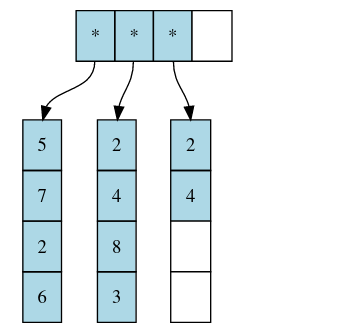
\includegraphics[width=0.55\textwidth]{ilustracije/hat-struktura-primer.png}
    \caption{Izgled stabla nizova koje redom sadrži brojeve 5, 7, 2, 6, 2, 4, 8, 3, 2 i 4}
    \label{fig:hat-struktura-primer}
\end{figure}

Za razliku od standardnih dinamičkih nizova, gde je sva alocirana memorija u jednom neprekidnom bloku, stablo nizova memoriju alocira u segmentima određene veličine. Iako ovaj pristup potencijalno kvari lokalnost referenci u \enquote{tačkama prekida} niza i uvodi dodatan nivo indirekcije pri pristupu elementima, on će omogućiti poboljšano iskorišćenje alocirane memorije.

Za potrebe implementacije osnovnih operacija nad ovom strukturom (umetanje elemenata, brisanje elemenata, indeksni pristup elementima), pored samih pokazivača potrebno je održavati i vrednosti koje predstavljaju trenutni broj elemenata, trenutni kapacitet (jednak sumi veličina alociranih korpi) i trenutni stepen stabla nizova, tj. broj $p$ takav da je veličina korpi jednaka $m = 2^p$. Osnovna struktura je prikazana u listingu \ref{lst:osnovna-struktura}.

U ostatku rada, stablo nizova će biti implementirano u programskom jeziku \verb|C++| u vidu klase \verb|hat_vector<T, Allocator>|. Svi kodovi će biti predstavljeni u pojednostavljenoj formi radi jednostavnije analize, a kompletna implementacija se može naći na \url{https://github.com/Aca-S/hashed-array-tree/}.

\begin{lstlisting}[language=C++, caption={Osnovna struktura stabla nizova}, captionpos=b, label={lst:osnovna-struktura}]
template <typename T, typename Allocator>
class hat_vector
{
    ...
    T** m_data; // Pokazivac na pocetak korenskog niza
    size_t m_power;     // Trenutni stepen stabla nizova
    size_t m_size;      // Trenutni broj elemenata
    size_t m_capacity;  // Trenutni kapacitet
    ...
};
\end{lstlisting}

\section{Analiza osnovnih operacija}

Kao što je slučaj i sa standardnim implementacijama strukture dinamičkog niza, stablo nizova pruža mogućnosti efikasnog umetanja elemenata na kraj i indeksnog pristupa elementima. Dodatno, pružene su i operacije umetanja elemenata na proizvoljnu poziciju, kao i brisanje elemenata sa proizvoljne pozicije.

\subsection{Pristup elementu po indeksu}

Da bi se u stablu nizova pristupilo nekom elementu po indeksu, prvo je potrebno naći list, tj. korpu kojoj pripada dati indeks, pa onda i tačnu poziciju koja odgovara indeksu unutar te korpe. Pošto su koren i sve korpe stabla iste veličine, redni broj odgovarajuće korpe se može dobiti kao količnik indeksa i veličine korpe, a pozicija unutar korpe kao ostatak pri deljenju indeksa i veličine korpe. S obzirom na to da je potrebno izvršiti samo ove dve operacije i onda pristupiti odgovarajućoj memorijskoj lokaciji, vremenska složenost pristupa elementu po indeksu je $O(1)$, tj. ne zavisi od broja elemenata u strukturi.

Iako je vremenska složenost indeksnog pristupa $O(1)$, on je i dalje poprilično skup usled upotrebe operacija deljenja i modula po veličini korpe. Iz ovog razloga, za veličinu korpi se obično uzimaju stepeni dvojke, jer to omogućava efikasnu implementaciju deljeja i modula po tom broju. Naime, neka je veličina korpe jednaka $m = 2^p$. Tada važi:
\begin{enumerate}
    \item \verb|pos / m = pos >> p|
    \item \verb|pos % m = pos & ((1 << p) - 1)|
\end{enumerate}
Prema tome, skupe operacije deljenja i modula se mogu zameniti jeftinim bitovskim operacijama. Implementacija ove operacije je prikazana u listingu \ref{lst:pristup-elementu}.

\begin{lstlisting}[language=C++, caption={Operacija pristupa elementu po indeksu \textit{pos}}, captionpos=b, label={lst:pristup-elementu}]
template <typename T, typename Allocator>
T& hat_vector<T, Allocator>::operator[](size_t pos)
{
    return m_data[pos >> m_power][pos & ((1 << m_power) - 1)];
}
\end{lstlisting}

\subsection{Dodavanje elementa na kraj}

U zavisnosti od trenutnog broja elemenata, kapaciteta i stepena stabla nizova, dodavanje elementa na kraj, pored upisa vrednosti na odgovarajuću memorijsku lokaciju, može zahtevati i povećanje stepena stabla i kopiranje svih prethodnih elemenata na nove memorijske lokacije i/ili alokaciju memorijskog prostora za novu korpu. Razmotrimo najgori slučaj, u kojem je potrebno izvršiti uvećanje stepena stabla, kroz primer dodavanja broja 4 na kraj kada imamo stablo nizova koje je prikazano na slici \ref{fig:dodavanje-na-kraj-primer-pocetak}.

\begin{figure}[h!]
    \centering
    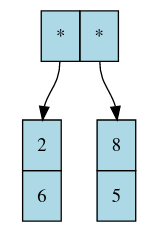
\includegraphics[width=0.3\textwidth]{ilustracije/dodavanje-na-kraj-primer-1.png}
    \caption{Puno stablo nizova stepena 1, tj. maksimalnog mogućeg kapaciteta 4}
    \label{fig:dodavanje-na-kraj-primer-pocetak}
\end{figure}

Ovo stablo je dostiglo maksimalan broj elemenata za svoj stepen, u ovom slučaju 4. Samo alociranje nove korpe nije moguće, pa je iz tog razloga prvo potrebno uvećati stepen stabla i time udvostručiti veličinu korena i korpi. Ovo se sprovodi alokacijom novog memorijskog prostora i kopiranjem svih elemenata iz starog stabla u novo stablo, stepena većeg za jedan. Novodobijeno stablo nizova za ovaj primer prikazano je na slici \ref{fig:dodavanje-na-kraj-primer-postupak} (a).

Po uvećanju stepena stabla nizova sa $p$ na $p + 1$, broj alociranih korpi u novom stablu biće jednak količniku broja elemenata u punom stablu stepena $p$ i veličine korpe u stablu stepena $p + 1$, tj. $\frac{2^{2p}}{2^{p + 1}} = 2^{p - 1}$. S obzirom na to da je ovaj količnik ceo broj, sve korpe dobijene uvećanjem stepena stabla biće popunjene do kraja, te je potrebno alocirati još jednu korpu za potrebe skladištenja elementa koji se dodaje na kraj, u ovom slučaju broja 4 - prikazano na slikama \ref{fig:dodavanje-na-kraj-primer-postupak} (b) i (c).

\begin{figure}[h!]
    \centering
    \subfigure[]{
        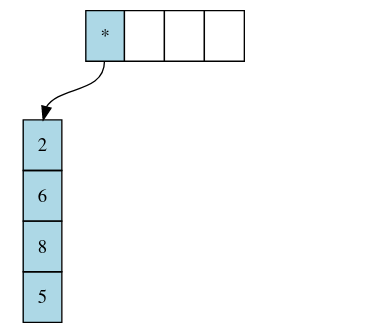
\includegraphics[width=0.3\textwidth]{ilustracije/dodavanje-na-kraj-primer-2.png}
    }
    \subfigure[]{
        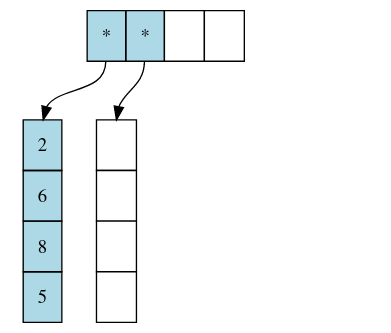
\includegraphics[width=0.3\textwidth]{ilustracije/dodavanje-na-kraj-primer-3.png}
    }
    \subfigure[]{
        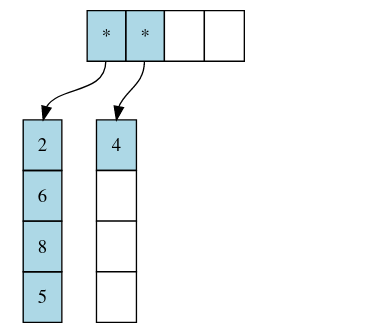
\includegraphics[width=0.3\textwidth]{ilustracije/dodavanje-na-kraj-primer-4.png}
    }
    \caption{Postupak dodavanja elementa na kraj}
    \label{fig:dodavanje-na-kraj-primer-postupak}
\end{figure}

Iako je, usled kopiranja svih elemenata, vremenska složenost prethodno opisanog najgoreg slučaja jednaka $O(n)$, gde je $n$ broj elemenata u stablu nizova, u najvećem broju slučajeva uvećanje stepena stabla neće biti potrebno. Naime, do ovog slučaja dolazi samo kada je broj elemenata, pre dodavanja još jednog, jednak $2^{2p}$, gde je $p$ trenutni stepen stabla nizova.

\begin{lemma}
Amortizovana složenost operacije dodavanja elementa na kraj stabla nizova je $O(1)$.
\end{lemma}

\begin{proof}
Pretpostavimo da, počev od praznog stabla nizova, dodajemo $n + 1$ elemenata na njegov kraj. Neka je, bez gubitka opštosti, $n = 2^{2p}$, gde je $p$ najmanji stepen stabla za koji ono može da sadrži $n$ elemenata. Tada za ukupan broj kopiranja elemenata važi
\begin{equation}
\begin{split}
    br\_kopiranja &= 2^{2p} + 2^{2(p - 1)} + 2^{2(p - 2)} + ... + 2^{2(p - p)} \\
    &= n + \frac{n}{4} + \frac{n}{16} + ... + \frac{n}{n} \\
    &< n + \frac{n}{4} + \frac{n}{16} + ... \\
    &= n(1 + \frac{1}{4} + \frac{1}{16} + ...) \\
    &= n \cdot \frac{4}{3}.
\end{split}
\end{equation}

Ukoliko za ukupnu cenu dodavanja $n + 1$ elemenata uzmemo zbir broja kopiranja i broja direktnih upisa vrednosti u memoriju (zanemarivši cenu alokacije pojedinačnih korpi, koja zavisi od konkretne strategije za alokaciju i stanja u memoriji), ukupna cena ovog procesa jednaka je $n + 1 + n \cdot \frac{4}{3}$. Prema tome, amortizovana cena dodavanja elementa na kraj jednaka je $\frac{n + 1 + n \cdot \frac{4}{3}}{n + 1} = O(1)$.
\end{proof}

\subsection{Umetanje elementa na proizvoljnu poziciju}

\subsection{Brisanje elementa sa proizvoljne pozicije}

\section{Analiza memorijske složenosti}

\section{Eksperimentalno merenje performansi}

\section{Zaključak}

\addcontentsline{toc}{section}{Literatura}
\appendix
\bibliography{literatura} 
\bibliographystyle{plain}

\end{document}
